\section{Baseline Paper}
\label{sec:baselinepaper}

To do justice to the contributions of \cite{tepNet2024}, it is addressed in a separate section highlighting the paper's specific insights and relevance. 
To the best of the author's knowledge, \cite{tepNet2024} is the only paper in the literature, which only filters out the two rails the train continuous on, presenting a solution to the rail track prediction problem.
Contrary to most literature, which filter out all rails, often without any distinction between rails, efforts in this direction have been made in \cite{RailraodSemanticPossibleTracks2020} and \cite{TPENet2023}.
However, because of the assumption that switch states cannot be accurately determined all "possible rail tracks" are considered in those two papers, leading to complex post-processing.
In \cite{tepNet2024}, the train's rails are defined as the "ego-path" and others are ignored.
To realize a system with this output \cite{tepNet2024} presents a novel regression-based approach, inspired by autonomous driving applications for road cars.

\vspace{0.5cm}

\noindent The main contributions of this work consist of several aspects.
First, unique annotations are created specifically for this project.
Furthermore, a data augmentation strategy is presented, incorporating two distinct cropping techniques for training and inference.
Additionally, a new Regression-based model architecture is developed, to meet the requirements of the novel problem formulation.
A custom loss function is introduced.
In the next few sections, each of these novelties is described in more detail.

\subsection{Annotations}

A new dataset is required for this. \cite{tepNet2024} works with its annotations and the RailSem19 dataset.
This dataset is in the so-called "ego-view", so the cameras are positioned in the driver's cabin and view the rails in front of the train.
For further details of the dataset utilized in this project, refer to section \ref{subsubsec:TEP-Net_dataset}.

\subsection{Data augmentation}

This section describes both the data augmentation strategy for training and the cropping augmentation for inference.

\subsubsection{Data augmentation for Training}

Three data augmentation techniques are implemented to train the model.
The first two are commonly used in CV tasks, including random horizontal flips and traditional image adjustments like brightness, contrast, saturation, and hue variations.
For this, the standard ColorJitter method from PyTorch is used \cite{pytorch_colorJitter_docu}.
The third augmentation is the cropping mechanism, which reduces the image to the most relevant part.
Randomness is also introduced to enhance generalization.

\autoref{fig:tepNet_dataaugmentation} visualizes the cropping algorithm steps schematically.
At first, there are two green lines, which follow the train's ego-path and represent the \ac{GT} in the form of polylines.
Then the yellow rectangle is computed with this information, being the smallest possible rectangle around the \ac{GT}.
In the next step, the orange box, the start pixels of the rails \ac{GT} are centered by expanding the yellow borders in one direction.
Important to mention is that in this tailored dataset the rails always begin in the first row at the bottom of each image.
After that margins are added shown by the red rectangle.
These margins are predefined with hyperparameters.
After calculating the borders of the outermost box variability is added to enhance generalization and prevent biases.
The left, right, and top borders are moved by a distance calculated with a normal distribution, which is defined by hyperparameters.
This introduced variability follows the policy, which ensures that the starting pixels of the rails at the bottom stay in the cropped image.
\autoref{fig:tepNet_dataaugmentation} illustrates four augmented variations of the top image in the bottom row.

\begin{figure}[H]
    \centering
    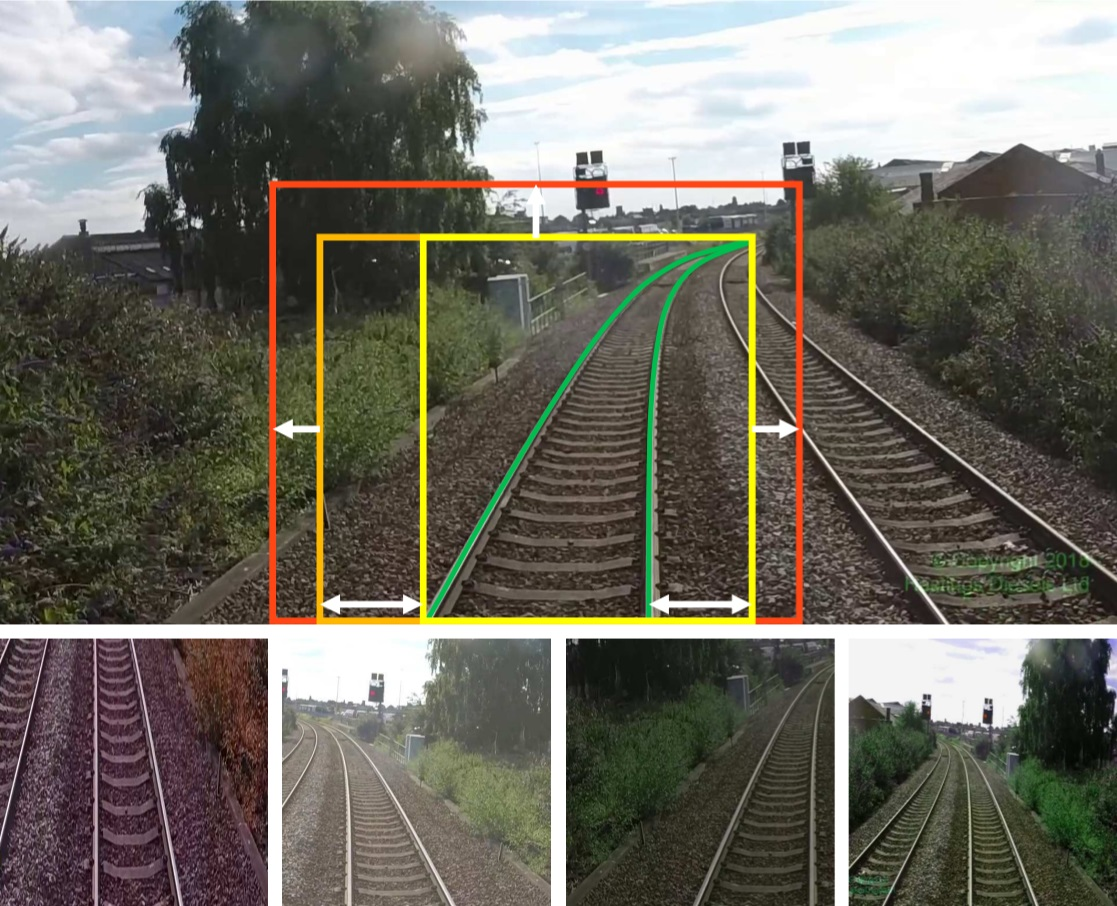
\includegraphics[width=\linewidth]{PICs/Baselinepaper/data_augmenation.jpg}
    \caption{Data augmentation of \ac{TEP}-Net \cite{tepNet2024}, including the image horizontal flips, the color variations and the cropping mechanism.}
    \label{fig:tepNet_dataaugmentation}
\end{figure}

\subsubsection{Cropping in inference}

In \cite{tepNet2024} only cropped images are used for training the model to minimize the images to their most relevant \ac{ROI}.
For training and validating the model on the dataset, the \ac{GT} allows the computation of crop coordinates (left, top, right).
However, \ac{GT} data is unavailable in practical applications like video inference.
As a result, the crop coordinates must be, either predefined by a user or computed on the fly.

In a real-world application the ROI in the images changes, even when the camera is mounted in a fixed position.
Because of these perspective shifts when the train drives right or left turns, it easily can become unsustainable to have predetermined crop coordinates.
\autoref{fig:perspective_shifts} visualizes these perspective shifts.
The tighter the curve, the worse the shift.
The approach of \cite{tepNet2024} to solve this particular problem is the so-called "Autocrop".
This developed technique starts with the whole image, so the initial crop cords are the image borders.
After the initialization, the three coordinates (left, top, right) are updated according to the prediction of every new frame.
In more detail, new coordinates are calculated with a running average of the smallest rectangle around the prediction plus the predefined margins from the training.

\begin{figure}[H]
    \centering
    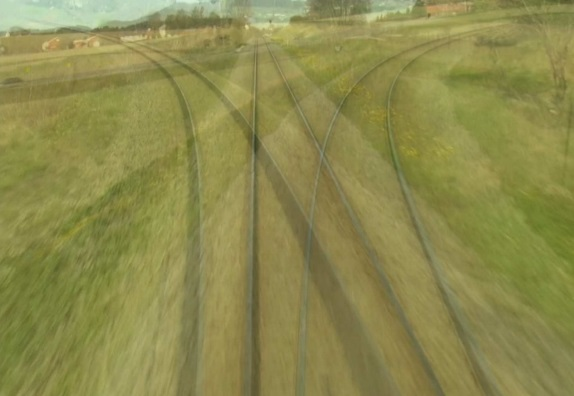
\includegraphics[width=\linewidth]{PICs/Baselinepaper/perspective_shifts.jpg}
    \caption{Example of perspective shifts with three different scenarios: left curve, right curve and straight rail \cite{tepNet2024}.}
    \label{fig:perspective_shifts}
\end{figure}

\subsection{TEP-Net Model}

In the literature, the particular problem of rail detection is usually solved with segmentation-based approaches.
One limitation of these approaches is the lack of distinction between all rails visible in the image and the rail the train continues.
The unique approach introduced by \cite{tepNet2024} takes a regression-based approach, which restricts the model to predict a single track.
The idea comes from various lane detection methods in autonomous driving applications for road cars and is fitted the rail domain.

Although rails can be represented by second or third-degree polynomials in curves, they may also take more complex geometric shapes.
Hence, limiting the output to presumed forms is discouraged.
Therefore, the method used in \cite{tepNet2024} employs spline interpolation to describe such complex structures.

\begin{figure}[H]
    \centering
    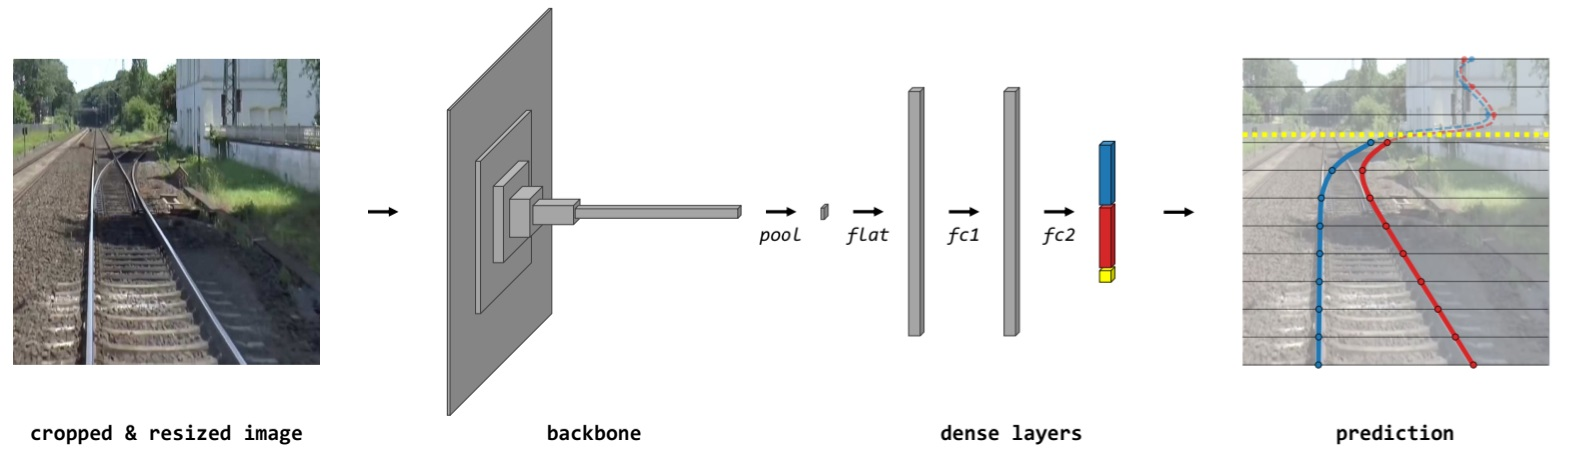
\includegraphics[width=\linewidth]{PICs/Baselinepaper/TEP-Net_model.jpg}
    \caption{\ac{TEP}-Net model architecture\cite{tepNet2024}. The input of the model is a cropped and resized image and the output of the model are the $x$-values for the left and right rail on each anchor line plus an additional value for the $y$-limit.}
    \label{fig:TEP-Net_model}
\end{figure}

As shown in the prediction of \autoref{fig:TEP-Net_model}, a set of horizontal lines are overlayed in the cropped image.
The number of $y$-lines or "anchors" is determined by a hyperparameter.
They are uniformly distributed along the $y$-axis. For each line, two $x$-values are predicted.
One for the left rail and one for the right rail.
The second and fourth images in the bottom row of \autoref{fig:tepNet_dataaugmentation} and the prediction image of \autoref{fig:TEP-Net_model} show that rails do not necessarily cross with anchor lines at the top of image crops.
Therefore, an additional $y$-limit is predicted, which gives information up to which anchor the rail should be detected.
Anchors and their $x$-values above this horizon line do not hold valuable information and are ignored.

For this novel regression task, a new model architecture is created.
For this model widely used backbone architectures like ResNet and EfficientNet are chosen.
These backbones extract relevant features from the cropped images reducing the spatial dimensions and increasing channel size to a high number.
After that, the feature map's number of channels is reduced to a predefined size with a 1x1 Conv2d layer \cite{pytorch_conv2d_docu} and flattened to a vector.
This feature vector serves as the input for the prediction head, which consists of two fully connected layers \cite{pytorch_linearLayer_docu} in series.
The size of the linear layers is set with a hyperparameter.
In the last layer, a reduction leads to the resulting prediction vector with the dimension $2 \times H + 1$.
$H$ is the number of anchors.
This vector includes the entire information of one prediction.
The first set of values with size $H$ is for the left rail, another $H$ set for the right rail and the $+ 1$ is for the last values being the horizon line.

This architecture's policy for value ranges does not restrict the $x$-values in any way.
This way predictions can be outside of a crop and the model can learn that sometimes the rails extend out of the viewed field.
The $y$-limit on the other hand is constrained to a range between 0 and 1 with a Sigmoid function.

The introduced model architecture can be classified as an end-to-end framework.
This means the model can be trained and used for inference without any steps in between.
It takes in raw data and results in a complete prediction.

\subsection{Loss function}

One of the main contributions of \cite{tepNet2024} is the loss function, which is tailored to the particular problem formulation of the regression-based approach.
The final loss function \autoref{func:combinedLoss} \cite{tepNet2024} consists of two sub-functions, where the outputs are added together, with the $y$-limit loss weighted by a multiplication factor of $\lambda=0.5$ before summing.

\begin{align}
    L = L_{traj} + \lambda \times L_{ylim}
    \label{func:combinedLoss}
\end{align}

The two sub-functions are the trajectory loss $L_{traj}$ and $y$-limit loss $L_{ylim}$.
For the following functions, $\hat{\mathbf{X}}$ and $\mathbf{X}$ represent the predicted and \ac{GT} $x$-values.
These include the points for the left and right rails.
For the $y$-limit, the predicted and \ac{GT} values are $\hat{y}_{lim}$ and $y_{lim}$.

\textbf{Trajectory Loss} $L_{traj}$ determines the error between the predicted and actual $x$-values.
To calculate this error, the sum of smoothL1 is used as shown in the numerator \autoref{func:trajectoryLoss}.
This is done with a $\beta_{1} = 0.005$. As shown in figure \autoref{fig:smoothL1}, this function allows a linearly proportional relationship between loss and error.
Additionally, for noise in the data, it includes a smooth transition at zero.

One issue of the front view perspective is the so-called linear perspective effect.
This effect occurs when rails continue into the distance.
The same pixel error represents a small distance when near the camera's capturing point and a larger distance when far away.
This ratio grows linearly the greater the distance to the camera.
To consider this effect, the results of the $L_{rails}(\hat{\mathbf{X}}_{i},\mathbf{X}_{i})$ are multiplied by the $w_{i}$ factor, which is inversely proportional to the width of the rail.
To prevent distortion of the results due to unreasonable weighting $W_{max}$ is used.
This value is the %95^{\text{th}}
percentile of all $w_{i}$ values from the training set.
This value is around 20 when data augmentation is used.

The $m_{i}$ factor is used to zero out and ignore all values above the $y$-limit.
Furthermore, it is ensured that the averaging of the loss is conducted exclusively over the relevant segment of the track.
This is done by summing all $m_{i}$ values in the denominator of \autoref{func:trajectoryLoss}.

%trajectory loss function
\begin{align}
    L_{traj} = \frac{\sum_{i=1}^H m_{i} \times w_{i} \times L_{rails}(\hat{\mathbf{X}}_{i},\mathbf{X}_{i})}
    {\sum_{i=1}^H m_{i}}
    \label{func:trajectoryLoss}
\end{align}

% smooth L1 error function
\begin{align}
    L_{rails} = \sum_{\substack{r \in \{left, right\}}} SmoothL1(\hat{\mathbf{X}}_{i,r} - \mathbf{X}_{i,r}, \beta_1)
    \label{func:smoothL1_error}
\end{align}

% Smooth L1
\begin{align}
    SmoothL1(x, \beta) = 
    \begin{cases}
        0.5 x^2 / \beta, & \text{if } |x| < \beta \\
        |x| - 0.5 * \beta, & \text{otherwise}
    \end{cases}
    \label{func:smoothL1}
\end{align}

% perspective weight function
\begin{align}
    w_{i} = \min \left( \frac{1}{\mathbf{X}_{i,right} - \mathbf{X}_{i,left}} , W_{max} \right)
    \label{func:perspective_weight}
\end{align}

% making factor
\begin{align}
    m_i = 
    \begin{cases} 
        1 & \text{if } i \leq y_{lim} \times H \\
        0 & \text{otherwise}
    \end{cases}
    \label{func:maskingFactor}
\end{align}

\textbf{Y-Limit Loss} $L_{ylim}$ is responsible for calculating the error of the horizon line.
For this sub-function also the $SmoothL1$ loss is taken with a $beta_{2} = 0.015$.
The value of $\beta_{2}$ is chosen to be higher, because of greater inaccuracy of annotations.
Due to images from the dataset stemming from low-resolution YouTube videos, it becomes difficult to accurately label the horizon line, especially when the end of the rail track is located at a significant distance.

\begin{align}
    L_{ylim} = SmoothL1(\hat{y_{lim}} - y_{lim}, \beta_{2})
    \label{func:ylimLoss}
\end{align}

\autoref{fig:smoothL1} shows a plot of the \autoref{func:smoothL1} because it is an important part of this loss function.

\vspace{1cm}

\begin{figure}[H]
    \centering
    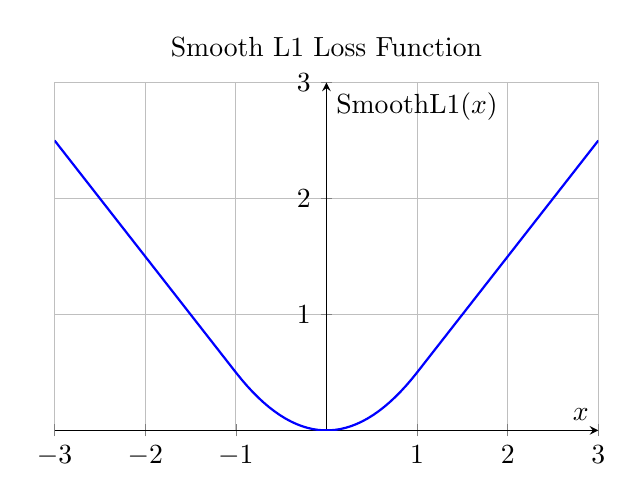
\begin{tikzpicture}
        \begin{axis}[
            title={Smooth L1 Loss Function},
            xlabel={$x$},
            ylabel={SmoothL1($x$)},
            grid=major,
            domain=-3:3, % Bereich der x-Achse
            samples=100, % Anzahl der Punkte
            axis lines=middle, % Achsen durch die Mitte
            %xmin=-3, xmax=3, % Zoom Bereich auf der x-Achse
            width=0.7\textwidth, % Breitere Grafik
            height=6cm, % Schmalere Höhe der Grafik
            ymin=0.0, ymax=3, % Zoom Bereich auf der y-Achse
        ]
            % SmoothL1-Funktion
            \addplot[
                blue, 
                thick
            %]{abs(x) < 0.005 ? 0.5 * (x^2) / 0.005 : abs(x) - 0.5 * 0.005};
            ]{(abs(x) < 1) * (0.5 * x^2) + (abs(x) >= 1) * (abs(x) - 0.5)};
        \end{axis}
    \end{tikzpicture}
    \caption{$SmoothL1$ Loss Funktion}
    \label{fig:smoothL1}
\end{figure}

\clearpage
\subsection{Experiments, Results and Comparison other state-of-the-art approaches of TEP-Net}

State-of-the-art approaches include two main ideas: a classification and a segmentation approach.
To fairly compare the novel regression-based architecture, \cite{tepNet2024} extends the model with two prediction heads, which support the two state-of-the-art methods.
For the segmentation model a U-Net-like \cite{uNet2015} decoder architecture is implemented, which outputs a binary mask with dimensions $1 \times 512 \times 512$.
A binary Dice loss is used for training.
The classification model is inspired by \cite{li2022rail}.
Therefore the prediction is also described in a grid system with the dimensions $C \times H \times (W + 1)$.
With $C=2$ for the number of rails, $H=64$ like the number of anchors in the regression model, and $W=128$ for the width of the grid following the settings from \cite{li2022rail}.
The $+1$ is for the background class.
Consequently, the classification model outputs a $2 \times 64 \times (128 + 1) = 16512$-dimensional vector.
A cross-entropy loss is used to train this model \cite{tepNet2024}.

For experiments, the same dataset is utilized.
With various preprocessing steps, the data annotation is transformed to fit the specific task of the model.
As described in \autoref{subsubsec:TEP-Net_dataset} the area between the rails is transformed into a binary mask for segmentation and the grid system is used for classification.
To get the most transparent comparison the same backbone is used for the three different models, as illustrated in \autoref{fig:TEP-Net_sota_models}.

\begin{figure}[H]
    \centering
    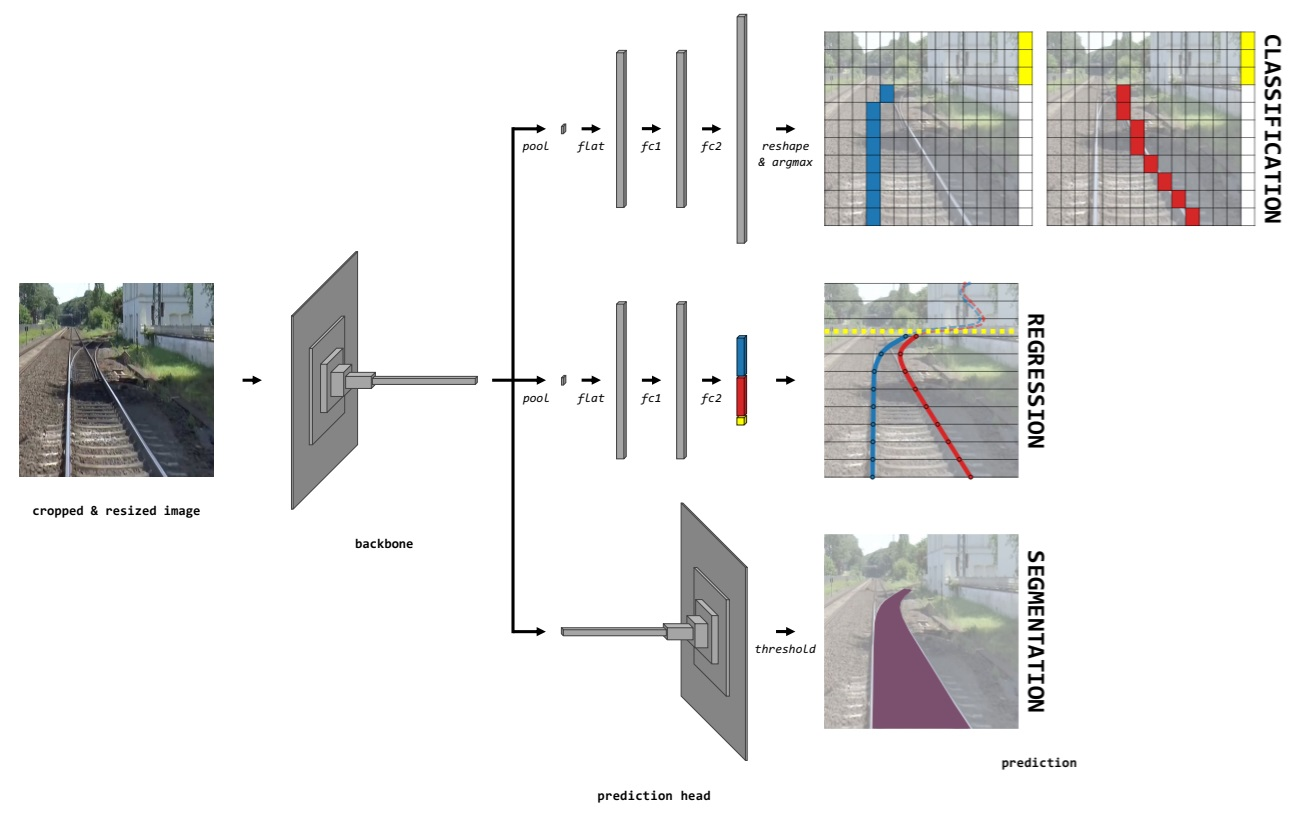
\includegraphics[width=\linewidth]{PICs/Baselinepaper/tep-net_sota_models.jpg}
    \caption{The model architecture is designed to enable a fair comparison between the novel regression model proposed in \cite{tepNet2024} and other \ac{SOTA} approaches.
    All models use the same dataset with preprocessing steps to fit annotation to the model task.}
    \label{fig:TEP-Net_sota_models}
\end{figure}

Experiments include trainings with different backbones: ResNet18, 34, 50 and EfficientNet B0, B1, B2, B3.
Results of \cite{tepNet2024} show that the segmentation-based approach is the most accurate when it comes to the \ac{IoU}.
However, the difference in \ac{IoU} performances is within a range of only 1.4 percent.
The segmentation model with the EfficientNet-B3 is the best and the classification model with the ResNet18 is the worst performing.
The Latency on the other hand shows that the segmentation model is the slowest.
Here the regression-based approach outperforms other models.
For the rail track prediction application of this work, the latency is of great importance.
Additionally, the regression model has lower numbers in parameters and \ac{MACs}, proving to be more lightweight compared to state-of-the-art models.
For more detailed results, please refer to \cite{tepNet2024}.

\begin{figure}[H]
    \centering
    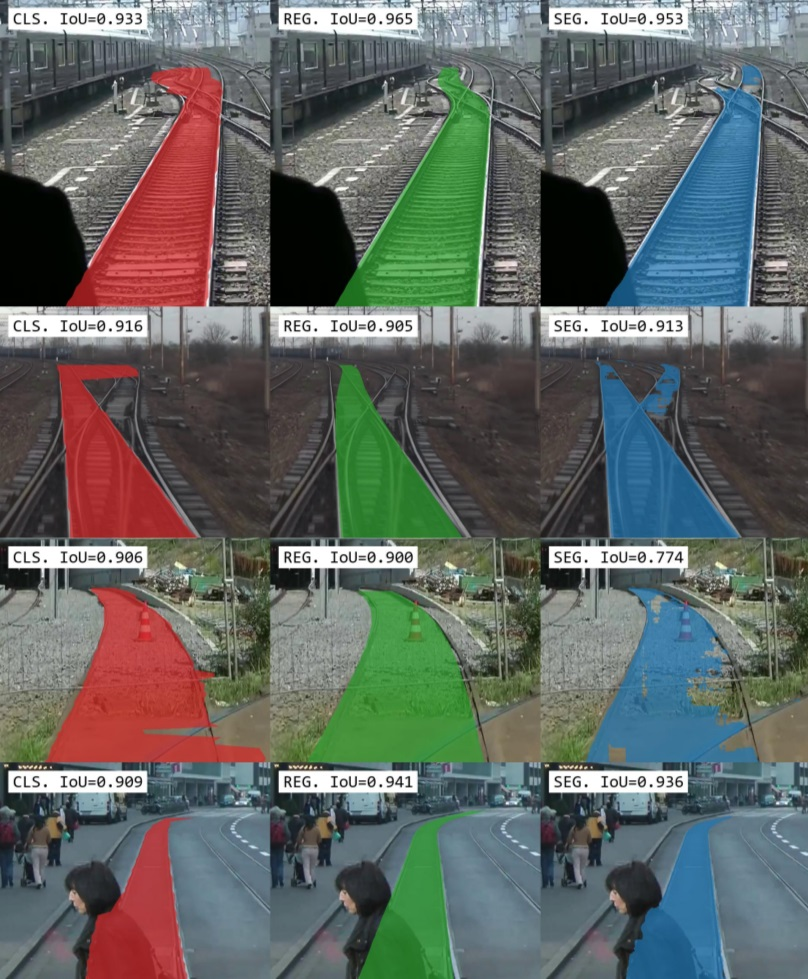
\includegraphics[width=0.7\linewidth]{PICs/Baselinepaper/comparison_sota_tep-net.jpg}
    \caption{Comparison between classification (CLS), regression (REG) and segmentation (SEG) models with challenging scenes.
    The ResNet18 backbone is used for this figure.}
    \label{fig:TEP-Net_sota_comparison}
\end{figure}

Since all three model architectures achieve similar \ac{IoU} scores, performances are compared on individual challenging scenes.
To see the differences more clearly the ResNet18 backbone is used because it is the worst performing in terms of accuracy.
As visualized in \autoref{fig:TEP-Net_sota_comparison}, the correctness of the prediction is negatively impacted when the model becomes unsure of where the rail track continues.
However, \autoref{fig:TEP-Net_sota_comparison} shows that the regression model is the only one that seems to have no issues with obstructions like in the lower two rows.
Additionally, when tracks split at upcoming switches, the novel approach of \cite{tepNet2024} is the only one that keeps the form of a rail.

This is due to the loss functions of both state-of-the-art models.
Both the dice loss and the cross-entropy loss penalize their models in the case of misclassification.
However, this penalty does not grow as the distance from the \ac{GT} increases.

The segmentation and the classification model work with probabilities, either on a pixel-wise or a grid-row level.
When segmentation models are confident, their pixel predictions tend toward the extremes of the output range.
Under uncertainty, they move closer to the middle which is also the threshold.
Similarly, classification models produce one-hot-like distributions when confident, but show more spread-out probabilities across classes when uncertain.
Since the regression approach inherently involves continuous values, the model assumes an average among the uncertain possibilities.
The concept of distance in the error between prediction and \ac{GT} is only provided in the regression-based model, but missing in segmentation and classification models.
Resulting in a more robust system \cite{tepNet2024}.

\subsection{Limitation}

The main limitation of \cite{tepNet2024} lies in its single-frame-based model architecture.
This model cannot capture temporal context, which becomes problematic when the train encounters a switch.
An example scenario is illustrated in \autoref{fig:limitationSwitch}.
Typically, the model effectively predicts the train's path when approaching switches, with all necessary information contained within the frame.
However, once the train passes over the switch and the start of the switch is no longer visible, the model cannot determine the continuation of the ego path.
Only after a certain duration, does the correct track become identifiable again.

\begin{figure}[H]
    \centering

    % Oberes Grid mit großen Bildern
    \begin{minipage}{0.328\textwidth}
        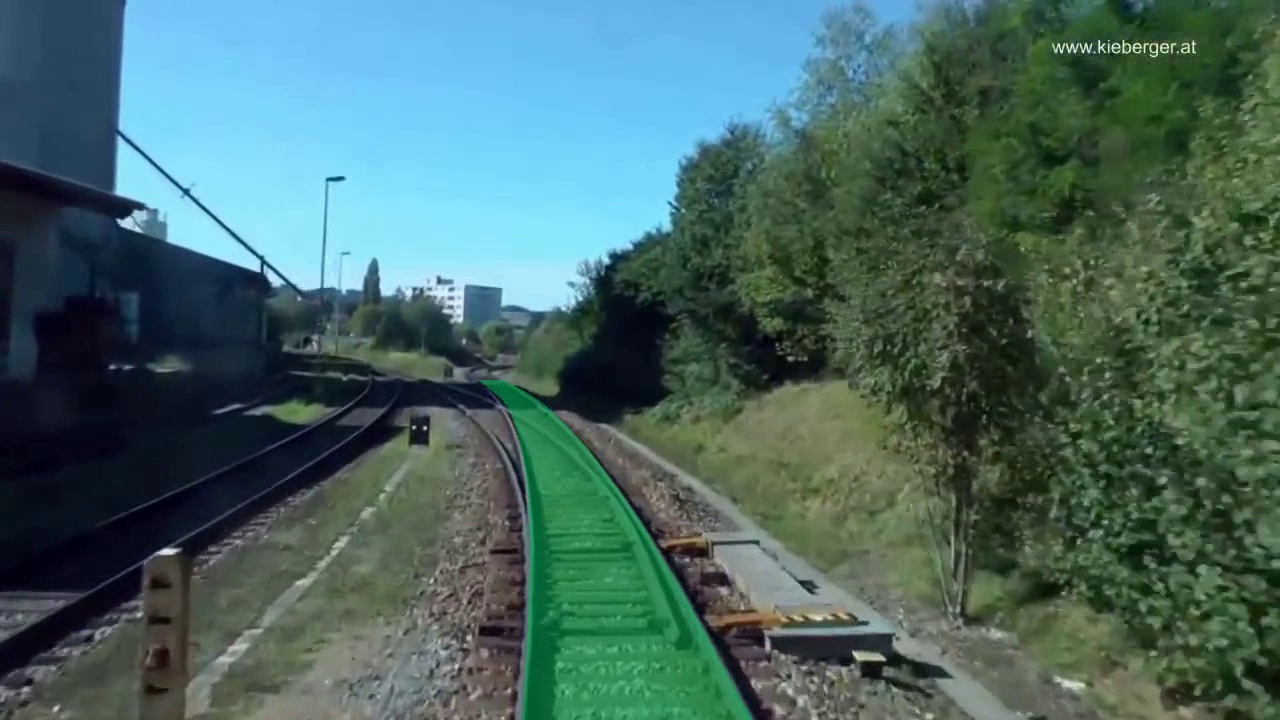
\includegraphics[width=\textwidth]{PICs/Baselinepaper/limitation_1.png}
    \end{minipage}
    \hfill
    \begin{minipage}{0.328\textwidth}
        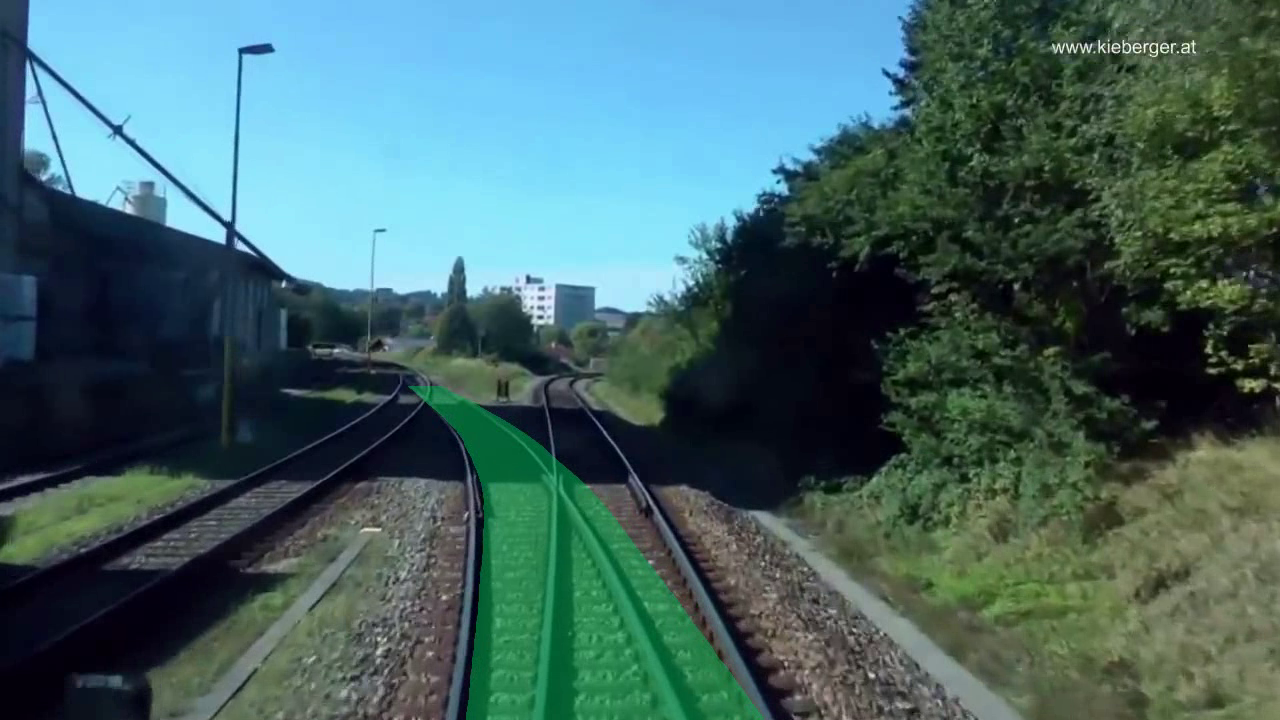
\includegraphics[width=\textwidth]{PICs/Baselinepaper/limitation_3.png}
    \end{minipage}
    \hfill
    \begin{minipage}{0.328\textwidth}
        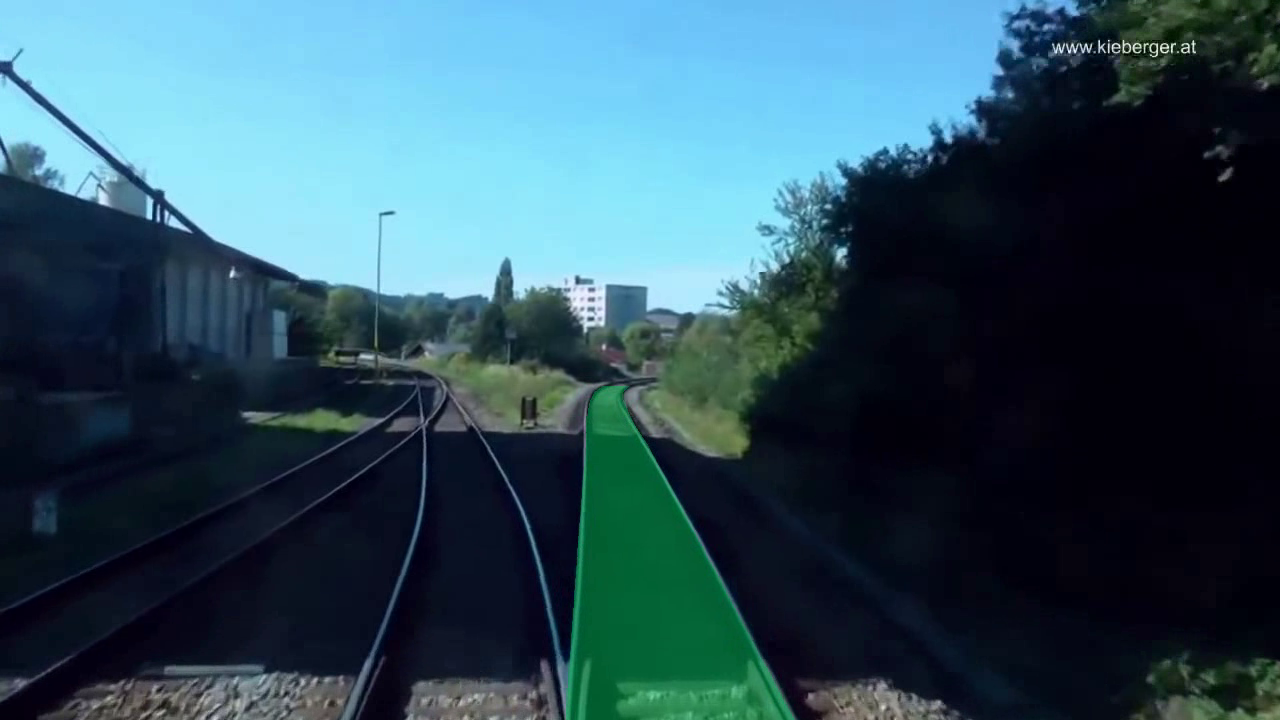
\includegraphics[width=\textwidth]{PICs/Baselinepaper/limitation_5.png}
    \end{minipage}

    \vspace{-0.15cm} % Kleinerer Abstand
    
    % Dritte Reihe nur für die Pfeile (zwischen oberen und unteren Bildern)
    \begin{minipage}{0.16\textwidth}
        \begin{tikzpicture}
            \node[anchor=south] (img) at (0,0) {};
            \draw[->, thick] (1.1,-0.1) -- (1.1,0.1); % Kürzerer Pfeil nach oben für das 1. Bild der unteren Reihe
        \end{tikzpicture}
    \end{minipage}
    \hfill
    \begin{minipage}{0.16\textwidth}
        % Kein Pfeil für dieses Bild
    \end{minipage}
    \hfill
    \begin{minipage}{0.16\textwidth}
        \begin{tikzpicture}
            \node[anchor=south] (img) at (0,0) {};
            \draw[->, thick] (0.5,-0.1) -- (0.5,0.1); % Kürzerer Pfeil nach oben für das 3. Bild der unteren Reihe
        \end{tikzpicture}
    \end{minipage}
    \hfill
    \begin{minipage}{0.16\textwidth}
        % Kein Pfeil für dieses Bild
    \end{minipage}
    \hfill
    \begin{minipage}{0.16\textwidth}
        \begin{tikzpicture}
            \node[anchor=south] (img) at (0,0) {};
            \draw[->, thick] (0.1,-0.1) -- (0.1,0.1); % Kürzerer Pfeil nach oben für das 5. Bild der unteren Reihe
        \end{tikzpicture}
    \end{minipage}
    \hfill
    \begin{minipage}{0.16\textwidth}
        % Kein Pfeil für dieses Bild
    \end{minipage}
    
    % Unteres Grid mit kleineren Bildern
    \begin{minipage}{0.16\textwidth}
        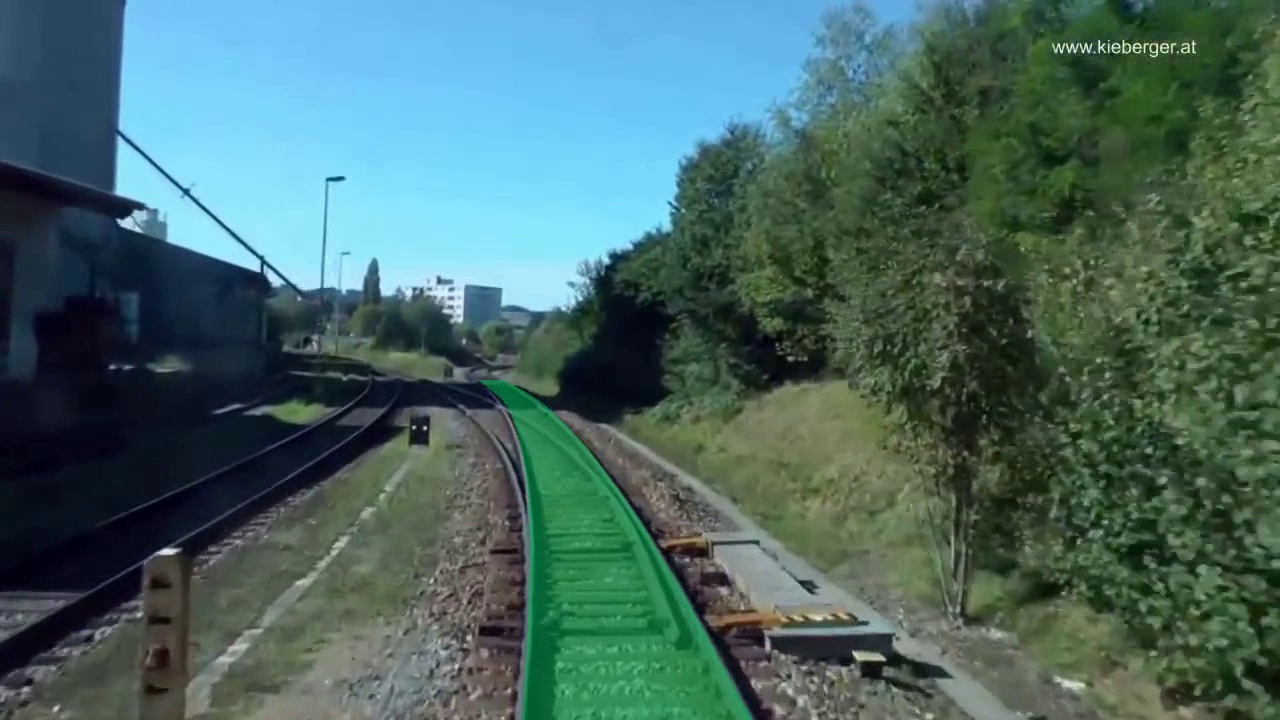
\includegraphics[width=\textwidth]{PICs/Baselinepaper/limitation_1.png}
    \end{minipage}
    \hfill
    \begin{minipage}{0.16\textwidth}
        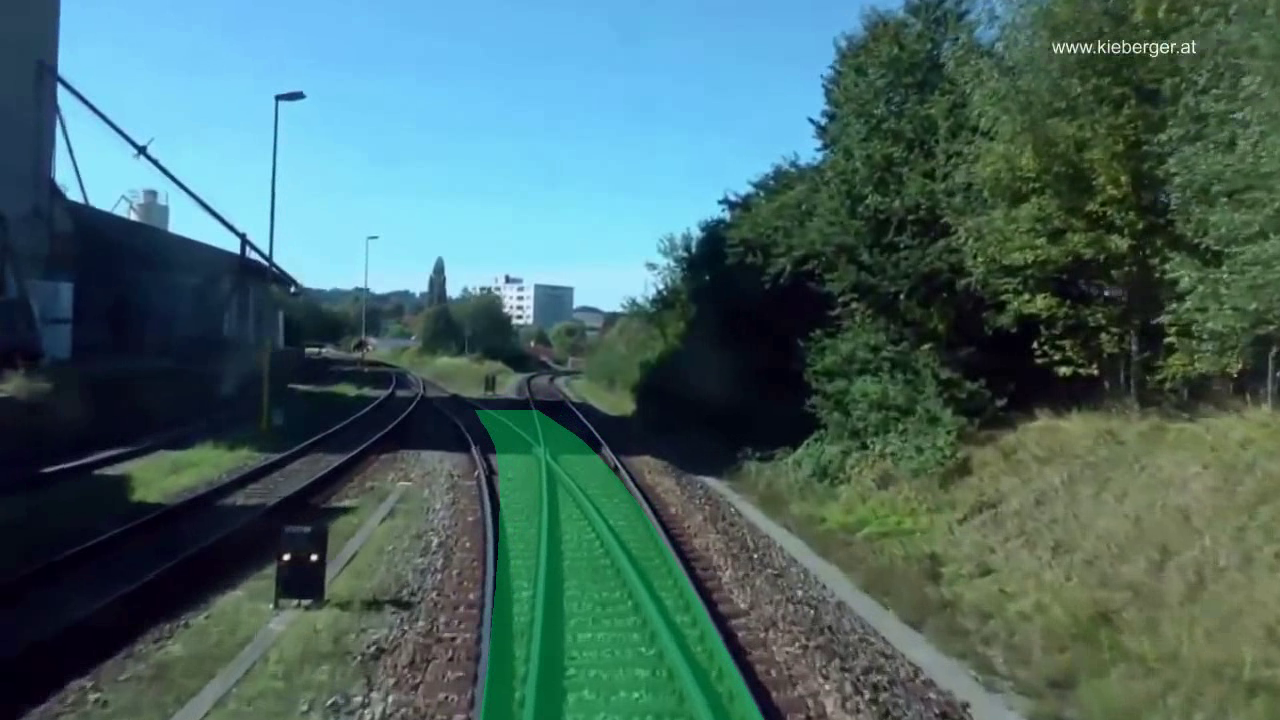
\includegraphics[width=\textwidth]{PICs/Baselinepaper/limitation_2.png}
    \end{minipage}
    \hfill
    \begin{minipage}{0.16\textwidth}
        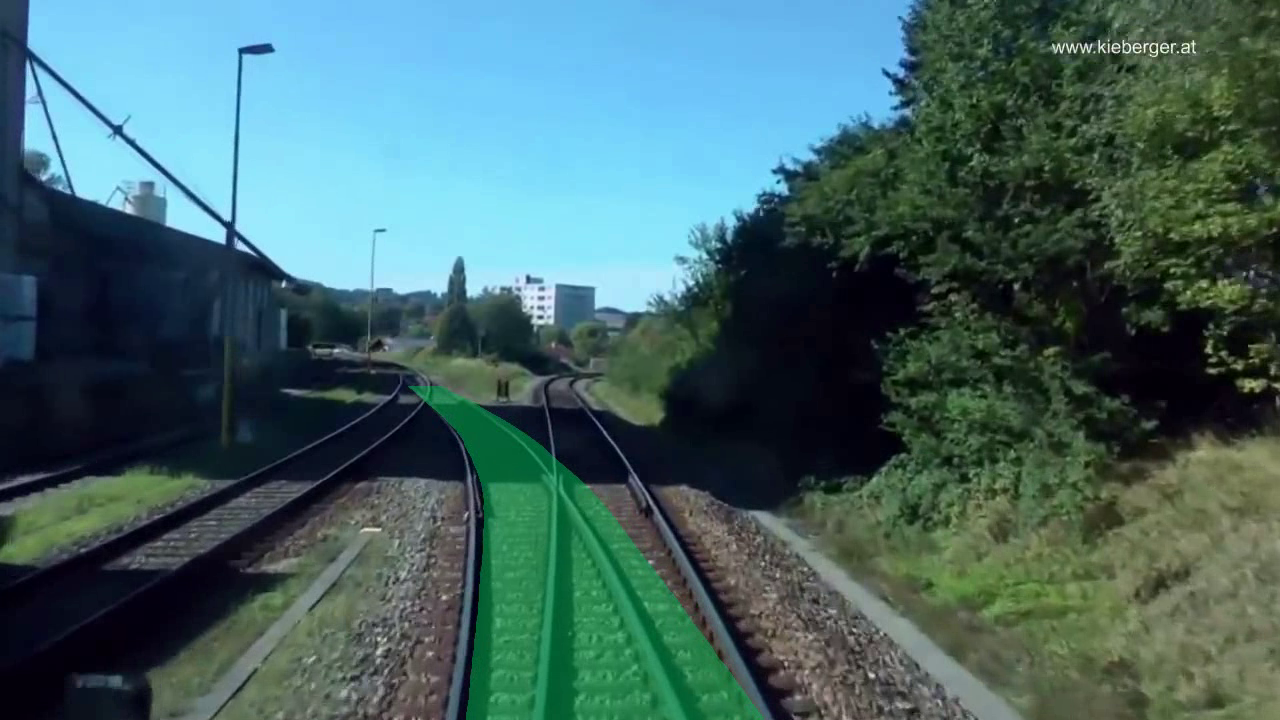
\includegraphics[width=\textwidth]{PICs/Baselinepaper/limitation_3.png}
    \end{minipage}
    \hfill
    \begin{minipage}{0.16\textwidth}
        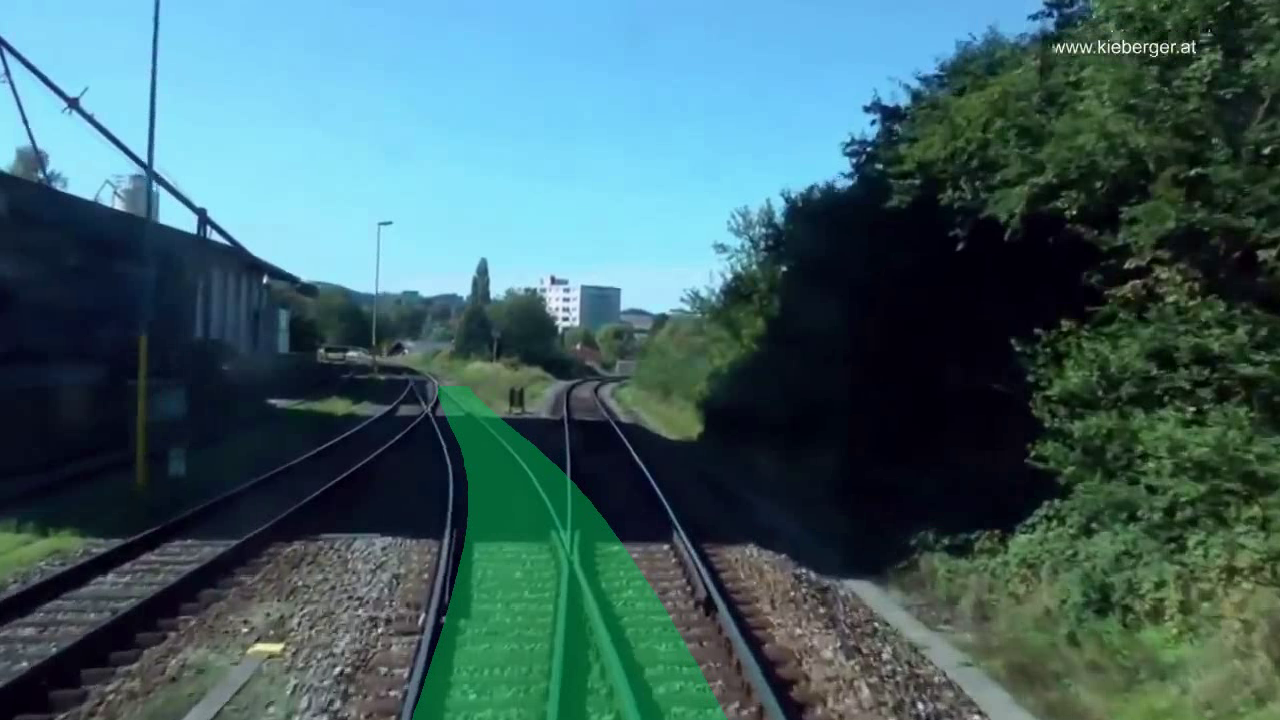
\includegraphics[width=\textwidth]{PICs/Baselinepaper/limitation_4.png}
    \end{minipage}
    \hfill
    \begin{minipage}{0.16\textwidth}
        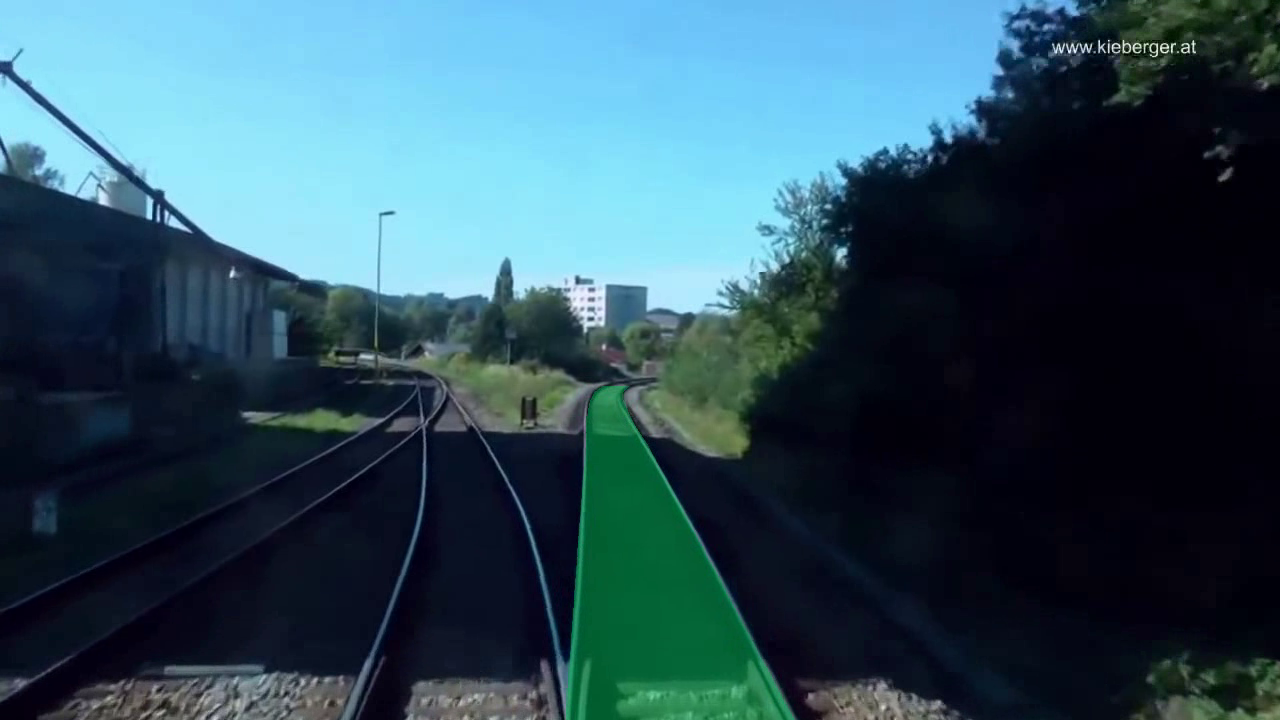
\includegraphics[width=\textwidth]{PICs/Baselinepaper/limitation_5.png}
    \end{minipage}
    \hfill
    \begin{minipage}{0.16\textwidth}
        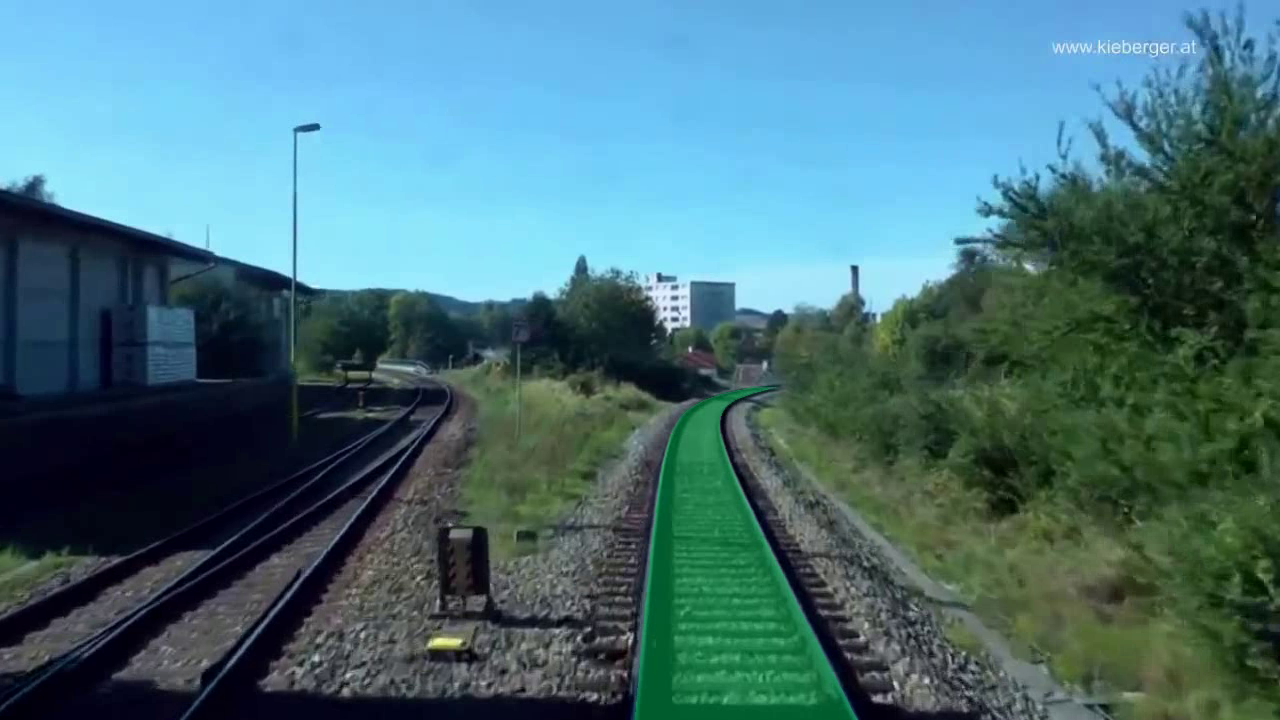
\includegraphics[width=\textwidth]{PICs/Baselinepaper/limitation_6.png}
    \end{minipage}

    % Vierte Reihe für die Zeitachse
    \begin{minipage}{1.0\textwidth}
        \centering
        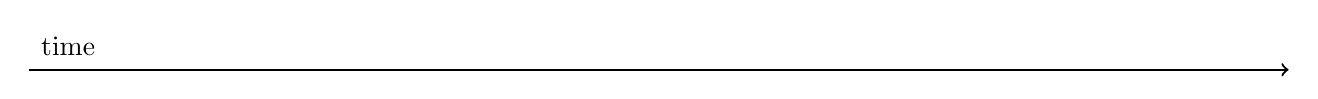
\begin{tikzpicture}
            % Zeit "Time" über dem Pfeil links positionieren
            \node at (-7.5, 0.3) {time}; % Text "Time"
            \draw[->, thick] (-8, 0) -- (8, 0); % Pfeil von ganz links nach ganz rechts
        \end{tikzpicture}
    \end{minipage}

    % Beschriftung unter dem Grid
    \vspace{0.5cm}
    \caption{Limitation of \ac{TEP}-Net \cite{tepNet2024}. The introduced approach is a single-frame-based model. Therefore, no temporal context can be captured, which leads to uncertainty in prediction when driving over a switch.
    All images are from \cite{limitaion_youtube_video}. A YouTube video, which is also used by RailSem19. It is ensured that none of the frames are included in the dataset, creating a fair test scenario.}
    \label{fig:limitationSwitch}
\end{figure}

There are two approaches suggested in \cite{tepNet2024}.
The first one includes integrating a confidence score to tell if the model is in a scenario where it is prone to become unreliable.
The second suggested approach is more complete.
It would encounter the temporal component by implementing a model like a \ac{RNN}, that can capture temporal information.
However, \cite{tepNet2024} states that there is no public temporal dataset available, which fits this task.
To the best of the author knowledge, this statement is correct.
Therefore, a corresponding dataset must also be created, if this approach is pursued.